\documentclass[border={10pt, 10pt, 10pt, 10pt}]{standalone}

\usepackage{tikz}
\usetikzlibrary{arrows}
\usetikzlibrary{decorations.markings}
\usepackage{standalone}

\begin{document}

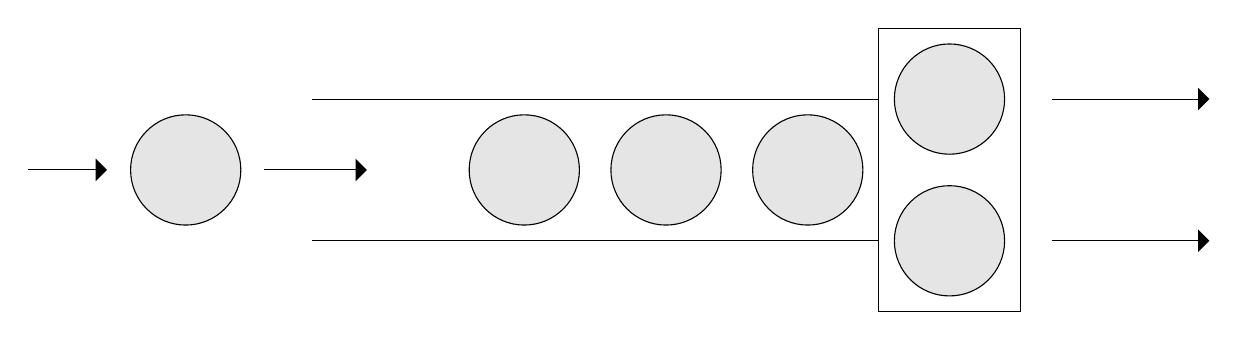
\begin{tikzpicture}



% Node top
\draw (2.1, 14.1) -- (9.3, 14.1) -- (9.3, 15.9) -- (2.1, 15.9);
\draw (9.3, 13.2) rectangle (11.1, 16.8);

% Top customers
\node[align=center] [style={minimum size=1.4cm, text width=1.0cm, draw=black,fill=black!10,text=black,shape=circle}] at (10.2, 15.9) {};
\node[align=center] [style={minimum size=1.4cm, text width=1.0cm, draw=black,fill=black!10,text=black,shape=circle}] at (10.2, 14.1) {};
\node[align=center] [style={minimum size=1.4cm, text width=1.0cm, draw=black,fill=black!10,text=black,shape=circle}] at (4.8, 15) {};
\node[align=center] [style={minimum size=1.4cm, text width=1.0cm, draw=black,fill=black!10,text=black,shape=circle}] at (6.6, 15) {};
\node[align=center] [style={minimum size=1.4cm, text width=1.0cm, draw=black,fill=black!10,text=black,shape=circle}] at (8.4, 15) {};
\draw[-triangle 90] (1.5, 15) -- (2.8, 15);
\draw[-triangle 90] (11.5, 15.9) -- (13.5, 15.9);
\draw[-triangle 90] (11.5, 14.1) -- (13.5, 14.1);

\draw[-triangle 90] (-1.5, 15) -- (-0.5, 15);
\node[align=center] [style={minimum size=1.4cm, text width=1.0cm, draw=black,fill=black!10,text=black,shape=circle}] at (0.5, 15) {};


\end{tikzpicture}

\end{document}
